\documentclass[5pt]{article}

\usepackage{sectsty}
\usepackage{graphicx}
\usepackage{lipsum} % for generating dummy text
\usepackage[margin=1in]{geometry}
\usepackage{setspace}
\usepackage{array}
\usepackage{cellspace}
\usepackage{tabularx}
\usepackage[table]{xcolor}
\usepackage{tabularray}
\usepackage{wrapfig}
\usepackage{flafter} 


\usepackage{hyperref}
\usepackage{scrextend}
\graphicspath{ {../assets} }


% Margins
\topmargin=-0.45in
\evensidemargin=0in
\oddsidemargin=0in
\textwidth=6.5in
\textheight=9.0in
\headsep=0.25in

\title{Analisi dei Requisiti}
\author{Jackpot Coding}
\renewcommand*\contentsname{Indice}
\renewcommand{\figurename}{Immagine}
\date{\today}

%longtblr
\DefTblrTemplate{contfoot-text}{default}{}
\DefTblrTemplate{conthead-text}{default}{}
\DefTblrTemplate{caption}{default}{}
\DefTblrTemplate{conthead}{default}{}
\DefTblrTemplate{capcont}{default}{}

%STARTOF THE DOCUMENT
\begin{document}

%-------------------------

% Reduce top margin only on the first page
\newgeometry{top=0.5in}

%UNIPD LOGO
    \vspace{8pt}
    
\includegraphics[scale=0.2]{UNIPDFull.png}
%END UNIPD LOGO

\vspace{30pt}

%COURSE INFO
\begin{minipage}[t]{0.48\textwidth}
    %COURSE TITLE
        \begin{flushleft}
            Informatica\\
            \vspace{5pt}
            \textbf{\LARGE Ingegneria del Software}\\
            Anno Accademico: 2023/2024
        \end{flushleft}
    %END COURSE TITLE
\end{minipage}
%END COURSE INFO


\vspace{5px}


%BLACK LINE
\rule{\textwidth}{5pt}

%JACKPOT CODING INFO
\begin{minipage}[t]{0.50\textwidth}
    %LOGO JACKPOT CODING
    \begin{flushleft}
        \hspace{10pt}
        
\includegraphics[scale=0.65]{jackpot-logo.png} 
    \end{flushleft}
\end{minipage}
\hspace{-60pt} % This adds horizontal space between the minipages
\begin{flushright}
    \begin{minipage}[t]{0.50\textwidth}
        %INFO JACKPOT CODING
        \begin{flushright}
            Gruppo: {\Large Jackpot Coding}\\
            Email: \href{mailto:jackpotcoding@gmail.com}{jackpotcoding@gmail.com}
        \end{flushright}
    \end{minipage}
\end{flushright}
%END JACKPOT CODING INFO

\vspace{24pt}

%TITLE
\begin{center}
    \textbf{\LARGE ANALISI DEI REQUISITI}
\end{center}
%END TITLE

\vspace{13pt}

\begin{flushleft}
    \begin{spacing}{1.5}
        REDATTORI: R. Simionato, G. Moretto, E. Gallo\\%INSERT HERE THE NAMES
        VERIFICATORI: G. Moretto, E. Gallo, R. Simionato\\
        \vspace{7pt}
        DESTINATARI: Prof. T. Vardanega, Prof. R. Cardin\\%INSERT HERE THE NAMES
    \end{spacing}
\end{flushleft}

\begin{flushright}
    \begin{spacing}{1}
        USO: ESTERNO\\
        VERSIONE: 1.0.0\\
    \end{spacing}
\end{flushright}


% Restore original margins from the second page onwards
\restoregeometry

\pagebreak

\textbf{\Large Registro delle modifiche}
\begin{longtblr}
	{
		colspec={|Q[0.10\linewidth]|Q[0.10\linewidth]|Q[0.15\linewidth]|Q[0.15\linewidth]|Q[0.45\linewidth]|},
		rows={halign=l},
		column{1}={halign=c},
		column{3}={halign=c},
		column{4}={halign=c},
		row{1}={halign=c},
		row{odd} = {gray!20},
		row{1}={teal!50},
	}
    \hline
    \textbf{Versione} & \textbf{Data} & \textbf{Autore} & \textbf{Verificatore} & \textbf{Modifica} \\
    \hline
    % versione & data & autore & verificatore & descrizioneModifica \\
    % \hline
    v.1.0.0 & 14/02/2024 & R. Simionato & G. Moretto & Approvazione \\
    \hline
    v.0.1.3 & 14/02/2024 & E. Gallo & R. Simionato & Aggiornata estetica del registro delle modifiche. Aggiunti Elenco delle immagini e Elenco delle tabelle\\
    \hline
    v.0.1.2 & 12/02/2024 & G.Moretto & E. Gallo & Aggiunti Tabella, Campi e Sinonimi  al glossario, correzione terminologia casi d'uso\\
    \hline
    v.0.1.1 & 12/02/2024 & G.Moretto & E. Gallo & Aggiunti riferimenti al Glossario \\
    \hline
    v.0.1.0 & 10/02/2024 & R. Simionato & G.Moretto & Verifica documento, aggiunta corsivo per termini in Inglese \\
    \hline
    v.0.0.14 & 11/01/2024 & R. Simionato & G.Moretto & Aggiunti Requisiti e Tracciamento \\
    \hline
    v.0.0.13 & 9/01/2024 & E. Gallo & G. Moretto & Aggiunti diagrammi UML per i casi d'uso \\
    \hline
    v.0.0.12 & 9/01/2024 & R. Simionato & G. Moretto & Aggiunta struttura tabelle dei Requisiti \\
    \hline
    v.0.0.11 & 9/01/2024 & R. Simionato & E. Gallo & Aggiunte sezioni Glossario e Riferimenti \\
    \hline
    v.0.0.10 & 8/01/2024 & E. Gallo & R. Simionato & Aggiunti UC 11. Modificati UC 7, 15.3, 16, 22, 30.2 \\
    \hline
    v.0.0.9 & 8/01/2024 & G. Moretto & E. Gallo & Aggiunti UC 26,28,28.1,28.2,30,30.1,30.2,31,32,32.1,32.2,33 \\
    \hline
    v.0.0.8 & 7/01/2024 & G. Moretto & E. Gallo & Aggiunti UC 5,7,11,17,19,21,22. Modificati UC 15, 15.1, 15.2, 15.3, 16, 16.1, 16.2, 16.3,18 \\
    \hline
    v.0.0.7 & 7/01/2024 & R. Simionato & G. Moretto & Aggiunti UC 11,12,14,15,17 \\
    \hline
    v.0.0.6 & 7/01/2024 & R. Simionato & G. Moretto & Aggiunti UC 18,19 alla struttura, diviso documento in sottofile \\
    \hline
    v.0.0.5 & 7/01/2024 & R. Simionato & G. Moretto & Aggiunti UC 3,4,7,8,9 e sottocasi  \\
    \hline
    v.0.0.4 & 5/01/2024 & R. Simionato & G. Moretto & Aggiunta nuova struttura per i Casi d'Uso \\
    \hline
    v.0.0.3 & 29/12/2023 & G. Moretto & R. Simionato  & Aggiunti UC 6,7,8,9,9.1,9.2, commentati altri \\
    \hline
    v.0.0.2 & 18/12/2023 & R. Simionato & G. Moretto & Aggiunte Introduzione, Descrizione e Casi d'uso \\
    \hline
    v.0.0.1 & 15/11/2023 & R. Simionato & G. Moretto  & Creata struttura del documento \\
  	\hline
\end{longtblr}



\pagebreak
\tableofcontents
\pagebreak
	\begin{flushleft}
\textbf{\Large Elenco delle immagini} 

\begin{spacing}{1.5} 

Immagine 1: Attori coinvolti \newline
Immagine 2: UC1,UC2 - Login \\
Immagine 3: UC1 - Inserimento nome utente e password \newline
Immagine 4: UC3,UC4 - Creazione struttura database \\
Immagine 5: UC3.1,UC3.2 - Inserimento nome e descrizione database \\
	Immagine 6: UC5 - Visualizzazione lista strutture database \\
	Immagine 7: UC6,UC7,UC8 - Visualizzazione, modifica ed eliminazione singola struttura database \\
	Immagine 8: UC9,UC10 - Creazione tabella \\
	Immagine 9: UC9,UC10 - Inserimento campi tabella \\
	Immagine 10: UC11 - Visualizzazione lista delle tabelle della struttura database \\
	Immagine 11: UC12,UC13,UC14 - Visualizzazione, modifica ed eliminazione della tabella \\
	Immagine 12: UC15,UC16 - Creazione campo tabella \\
	Immagine 13: UC15,UC16 - Inserimento singolo campo tabella \\
	Immagine 14: UC17 - Visualizzazione lista dei campi della tabella \\
	Immagine 15: UC18,UC19,UC20 - Visualizzazione, modifica ed eliminazione singolo campo tabella \\
	Immagine 16: UC21,UC22 - Caricamento struttura database tramite file \\
	Immagine 17: UC23,UC24 - Logout \\
	Immagine 18: UC25,UC26 - Selezione struttura database \\
	Immagine 19: UC27,UC28 - Inserimento frase in linguaggio naturale \\
	Immagine 20: UC28 - Errore frase inserita \\
	Immagine 21: UC29,UC30 - Visualizzazione prompt generato \\
	Immagine 22: UC30 - Errore comunicazione con LLM \\
	Immagine 23: UC31,UC32 - Richiesta generazione query SQL \\
	Immagine 24: UC32 - Errore comunicazione con API 
\end{spacing}
\end{flushleft}


\pagebreak

\begin{flushleft}
\textbf{\Large Elenco delle tabelle}
\begin{spacing}{1.5}

	Tabella 1: Requisiti funzionali \\
	Tabella 2: Requisiti di qualità \\
	Tabella 3: Requisiti di vincolo \\
	Tabella 4: Fonte-Requisiti \\
	Tabella 5: Requisito-Fonti \\
	Tabella 6: Riepilogo
\end{spacing}
\end{flushleft}

\pagebreak

\section{Introduzione}
\subsection{Scopo del documento}
Questo documento serve a fornire una descrizione dettagliata del funzionamento del prodotto, prestando particolare attenzione a come il prodotto potrà essere usato e a quanto richiesto dai requisiti presentati e discussi con il proponente.
Analizzando questi cerchiamo quindi di individuare ed illustrare i diversi attori e i casi d’uso presenti all’interno del prodotto.\\
Ogni caso d’uso rappresenta uno scenario di utilizzo del programma da parte di un attore, per descriverlo al meglio utilizzeremo la struttura seguente:
\begin{itemize}
	\item Descrizione: breve descrizione del caso d'uso;
	\item Attori: chi esegue l'azione descritta;
	\item Precondizioni: stato del programma prima del caso d'uso;
	\item Postcondizioni: stato del programma dopo il caso d'uso;
	\item Scenario principale: azioni svolte prima, durante e dopo il caso d'uso;
	\item Generalizzazioni: se presenti, scomposizione del caso d'uso in sottocasi;
	\item Estensioni: se presenti, casi d'uso collegati(es. visualizzazione di errori o avvisi).
\end{itemize}
Ogni attore rappresenta una persona o un sistema esterno al programma che si interfaccia con esso.
Nel nostro caso il programma verrà utilizzato da due tipi di attori che avranno accesso a diverse funzionalità del prodotto:
\begin{itemize}
	\item \textbf{Utente}: può scegliere il database a cui fare la richiesta e inserire il messaggio in linguaggio naturale che verrà utilizzato per la creazione del prompt;
	\item \textbf{Amministratore}: può aggiungere, modificare e eliminare i database selezionabili dagli utenti.
\end{itemize} % __DA VERIFICARE__ decidere se lasciare la descrizione degli attori qui o se spostarla

\subsection{Glossario}
Al fine di evitare incomprensioni riguardo la terminologia usata e per aiutare la comprensione del documento, viene fornito un Glossario nel file omonimo con la definizione precisa di ogni vocabolo potenzialmente ambiguo. Su questi termini verrà apposta un G in pedice per indicare la presenza della definizione nel Glossario.

\subsection{Riferimenti}
\subsubsection{Riferimenti normativi}
\begin{itemize}
	\item Capitolato C9 - ChatSQL \\ \url{https://www.math.unipd.it/~tullio/IS-1/2023/Progetto/C9.pdf}
	\item Norme di progetto
\end{itemize}

\subsubsection{Riferimenti informativi}
\begin{itemize}
	\item Slide T5 - Analisi dei requisiti - Corso di Ingegneria del Software \\ \url{https://www.math.unipd.it/~tullio/IS-1/2023/Dispense/T5.pdf}
	\item Diagrammi dei casi d'uso - Corso di Ingegneria del Software \\ \url{https://www.math.unipd.it/~rcardin/swea/2022/Diagrammi%20Use%20Case.pdf}
\end{itemize}

\section{Descrizione}
\subsection{Obiettivi del prodotto}
Il prodotto ha come obiettivo di dare la possibilità di interrogare un database partendo da una richiesta in linguaggio naturale e trasformandola in un prompt da sottoporre ad un sistema di AI per ottenere una query SQL corretta in base alla struttura del database interrogato.

\subsection{Funzioni del prodotto}
Il prodotto dovrà quindi, dati:
\begin{itemize}
	\item un file strutturato contenente le tabelle e le relazioni di un database;
	\item una frase in linguaggio naturale per interrogare suddetto database.
\end{itemize}
Trovare nella frase le parole chiave, capendo quali sono i dati da visualizzare, in quali tabelle sono salvate, tenendo conto di eventuali condizioni imposte.
In seguito riscrivere la frase in modo da generare un prompt che possa essere passato ad un sistema AI che creerà la query richiesta in linguaggio SQL.
Il prompt generato potrà essere semplicemente mostrato all’utente, che sarà tenuto ad inserirlo nel sistema AI da lui scelto, oppure utilizzare le API delle AI per sottoporre direttamente il prompt e mostrare all’utente il codice SQL.
Il prodotto dovrà inoltre dare la possibilità agli utenti amministratori, dopo aver effettuato l’accesso, di:
\begin{itemize}
	\item aggiungere file strutturati selezionabili dagli utenti;
	\item modificare i file strutturati;
	\item eliminare file strutturati non più necessari.
\end{itemize}

\section{Casi d'uso}
% TEMPLATE
%   \subsection{UC - NomeUseCase}
%   \label{sec:UC}
%   \includegraphics[]{diagramma_UML}
%   \begin{itemize}
	%       \item \textbf{Descrizione:} 
	%       \item \textbf{Attori:} 
	%       \item \textbf{Precondizioni:} 
	%       \item \textbf{Postcondizioni:} 
	%       \item \textbf{Scenario principale:} 
	%       \item \textbf{Generalizzazioni:} 
	%       \item \textbf{Estensioni:} 
	%   \end{itemize}

%   \hyperref[sec:UC]{\textbf{UC}}

% Link ad altre sezioni usando hyperref - utile per linkare generalizzazioni e estensioni
% La label fa da segnalibro a dove dovrà andare il link
%   \label{sec:nomeSezione}
% Link sul quale cliccare per andare alla label
%   \hyperref[sec:nomeSezione]{testo}
% END TEMPLATE

\subsection{Obiettivi}
La sezione ha come obiettivo quello di identificare e descrivere tutti i casi d'uso che sono stati individuati dal gruppo in sede di analisi del capitolato assegnato.

\subsection{Attori}
\begin{wrapfigure}{r}{3.5cm}
	
\includegraphics[width=3.5cm]{UML_Use_Cases/UC-Attori.png}
\end{wrapfigure}
Il sistema dispone di due attori principali. In particolare:
\begin{itemize}
	\item \textbf{Utente}, che accede al servizio come utente in grado di selezionare una struttura \textit{database} precaricata, inserire una frase di interrogazione in linguaggio naturale, visualizzare il \textit{prompt} generato dall'\textit{LLM} per poi confermarlo e ottenere una frase in formato \textit{SQL} che rappresenti quello che era stato richiesto inizialmente.
	\item \textbf{Amministratore}, generalizzazione dell'utente generico, accede al servizio come amministratore. Oltre a poter compiere tutte le azioni che può fare l'utente generico, l'amministratore può creare, visualizzare, modificare ed eliminare un \textit{database}, le sue tabelle e i suoi campi.
\end{itemize}
% 
\includegraphics[scale=0.6]{UML_Use_Cases/UC-Attori.png}

\setcounter{secnumdepth}{0}

\subsection{UC1 - \textit{Login}}
\label{sec:UC1}
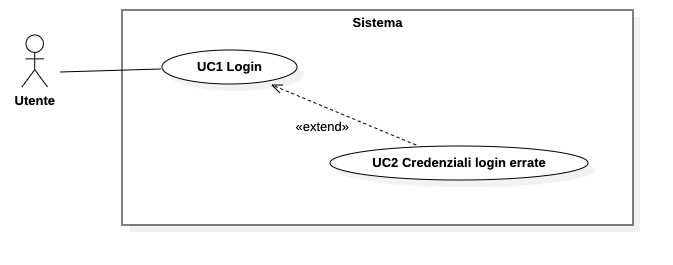
\includegraphics[scale=0.6]{UML_Use_Cases/UC1_2.png}
\begin{itemize}
	\item \textbf{Descrizione:} L’amministratore accede al pannello amministrativo con le sue credenziali;
	\item \textbf{Attori:} amministratore;
	\item \textbf{Precondizioni:} 
	\begin{itemize}
		\item L’amministratore possiede delle credenziali di accesso valide;
		\item L’amministratore non ha già effettuato l’accesso;
	\end{itemize}
	\item \textbf{Postcondizioni:} 
	\begin{itemize}
		\item L’utente Amministratore viene riconosciuto dal sistema;
	\end{itemize}
	\item \textbf{Scenario principale:} 
	\begin{itemize}
		\item L’ amministratore inserisce il proprio nome utente nel form di accesso (\hyperref[sec:UC1.1]{\textbf{UC1.1}});
		\item L’ amministratore inserisce la propria password nel form di accesso (\hyperref[sec:UC1.2]{\textbf{UC1.2}});
		\item Il sistema verifica che le credenziali ricevute siano corrette. 
	\end{itemize}
	\item \textbf{Estensioni:} Nel caso le credenziali non siano corrette:
	\begin{itemize}
		\item viene mostrato un errore - \hyperref[sec:UC2]{\textbf{UC2}}
	\end{itemize}
\end{itemize}

\subsubsection{UC1.1 - Inserimento nome utente}
\label{sec:UC1.1}
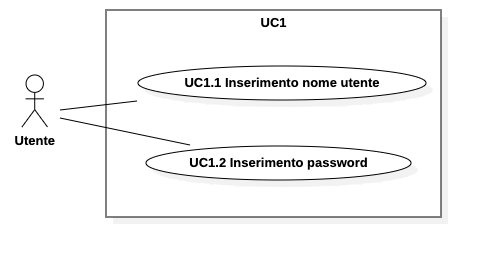
\includegraphics[scale=0.6]{UML_Use_Cases/UC1.1_1.2.png}
\begin{itemize}
	\item \textbf{Descrizione:} L’amministratore inserisce il proprio nome utente;
	\item \textbf{Attori:} amministratore;
	\item \textbf{Precondizioni:} 
	\begin{itemize}
		\item L’amministratore possiede le credenziali di accesso;
		\item L’amministratore non ha già effettuato l’accesso;
		\item L’amministratore sta effettuando il \textit{login} (\hyperref[sec:UC1]{\textbf{UC1}})
	\end{itemize}
	\item \textbf{Postcondizioni:} 
	\begin{itemize}
		\item L’amministratore ha inserito correttamente il proprio nome utente;
	\end{itemize}
	\item \textbf{Scenario principale:} 
	\begin{itemize}
		\item L’amministratore inserisce il proprio nome utente nel form di accesso.
	\end{itemize}
\end{itemize}

\subsubsection{UC1.2 - Inserimento password}
\label{sec:UC1.2}
%\includegraphics[]{diagramma_UML}
\begin{itemize}
	\item \textbf{Descrizione:} L’amministratore inserisce la propria password;
	\item \textbf{Attori:} amministratore;
	\item \textbf{Precondizioni:} 
	\begin{itemize}
		\item L’amministratore possiede le credenziali di accesso;
		\item L’amministratore non ha già effettuato l’accesso;
		\item L’amministratore sta effettuando il \textit{login} (\hyperref[sec:UC1]{\textbf{UC1}})
	\end{itemize}
	\item \textbf{Postcondizioni:} 
	\begin{itemize}
		\item L’amministratore ha inserito correttamente la propria password;
	\end{itemize}
	\item \textbf{Scenario principale:} 
	\begin{itemize}
		\item L’amministratore inserisce la propria password nel form di accesso.
	\end{itemize}
\end{itemize}

\subsection{UC2 - Credenziali \textit{login} errate}
\label{sec:UC2}
%\includegraphics[]{diagramma_UML}
\begin{itemize}
	\item \textbf{Descrizione:} L’amministratore visualizza un messaggio di errore di autenticazione;
	\item \textbf{Attori:} amministratore;
	\item \textbf{Precondizioni:} 
	\begin{itemize}
		\item L’amministratore possiede le credenziali di accesso;
		\item L’amministratore non ha già effettuato l’accesso;
		\item L’amministratore sta effettuando il \textit{login} (\hyperref[sec:UC1]{\textbf{UC1}});
		\item L’amministratore ha inserito il proprio nome utente (\hyperref[sec:UC1.1]{\textbf{UC1.1}});
		\item L’amministratore ha inserito la propria password (\hyperref[sec:UC1.2]{\textbf{UC1.2}});
	\end{itemize}
	\item \textbf{Postcondizioni:}
	\begin{itemize}
		\item L’amministratore non viene riconosciuto dal sistema e deve reinserire le proprie credenziali;
		\item L'amministrazione visualizza un messaggio di errore;
	\end{itemize}
	\item \textbf{Scenario principale:} 
	\begin{itemize}
		\item Il sistema verifica le credenziali ricevute siano corrette;
		\item Il sistema visualizza un messaggio di errore per le credenziali inserite se non corrette.
	\end{itemize}
\end{itemize}

\subsection{UC3 - Creazione \textit{Database}}
\label{sec:UC3}
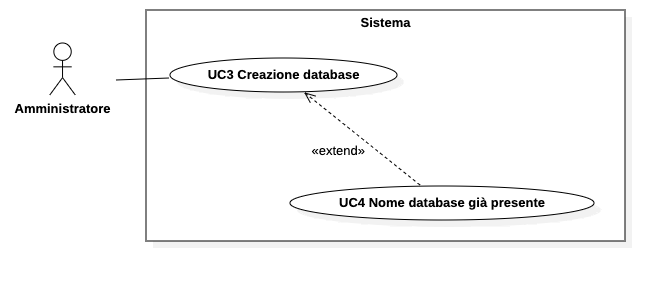
\includegraphics[scale=0.6]{UML_Use_Cases/UC3_4.png}
\begin{itemize}
	\item \textbf{Descrizione:} l’amministratore vuole aggiungere la struttura di un \textit{database} da poter interrogare;
	\item \textbf{Attori:} amministratore;
	\item \textbf{Precondizioni:} 
	\begin{itemize}
		\item L’amministratore ha effettuato il \textit{login} (\hyperref[sec:UC1]{\textbf{UC1}});
		\item L’amministratore si trova nel pannello amministrativo;
	\end{itemize}
	\item \textbf{Postcondizioni:} 
	\begin{itemize}
		\item La struttura del \textit{database} viene salvata nel programma;
	\end{itemize}
	\item \textbf{Scenario principale:} 
	\begin{itemize}
		\item L’amministratore inserisce il nome (\hyperref[sec:UC3.1]{\textbf{UC3.1}}) e la descrizione (\hyperref[sec:UC3.2]{\textbf{UC3.2}}) del \textit{database};
	\end{itemize}
	\item \textbf{Estensioni:} nel caso in cui venga inserito un nome già esistente:
	\begin{itemize}
		\item \hyperref[sec:UC4]{\textbf{UC4}} - Errore: nome \textit{Database} già presente
	\end{itemize}
\end{itemize}

\subsubsection{UC3.1 - Inserimento nome \textit{Database}}
\label{sec:UC3.1}
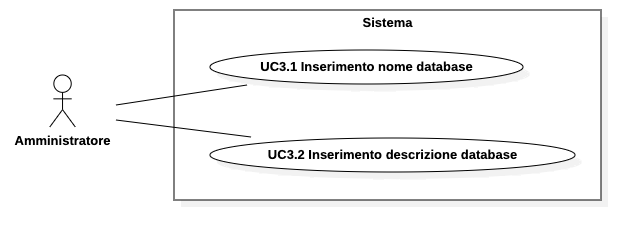
\includegraphics[scale=0.6]{UML_Use_Cases/UC3.1_3.2.png}
\begin{itemize}
	\item \textbf{Descrizione:} l’amministratore deve inserire il nome del nuovo \textit{database} da aggiungere;
	\item \textbf{Attori:} amministratore;
	\item \textbf{Precondizioni:} 
	\begin{itemize}
		\item L’amministratore ha effettuato il \textit{login} (\hyperref[sec:UC1]{\textbf{UC1}});
		\item L’amministratore si trova nel pannello amministrativo;
		\item L’amministratore sta creando un nuovo \textit{database} (\hyperref[sec:UC3]{\textbf{UC3}});
	\end{itemize}
	\item \textbf{Postcondizioni:} 
	\begin{itemize}
		\item L'amministratore ha inserito correttamente il nome del nuovo \textit{database};
	\end{itemize}
	\item \textbf{Scenario principale:} 
	\begin{itemize}
		\item L’amministratore inserisce il nome del \textit{database};
	\end{itemize}
\end{itemize}

\subsubsection{UC3.2 - Inserimento descrizione \textit{Database}}
\label{sec:UC3.2}
%\includegraphics[]{diagramma_UML}
\begin{itemize}
	\item \textbf{Descrizione:} l’amministratore deve inserire la descrizione del nuovo \textit{database} da aggiungere;
	\item \textbf{Attori:} amministratore;
	\item \textbf{Precondizioni:} 
	\begin{itemize}
		\item L’amministratore ha effettuato il \textit{login} (\hyperref[sec:UC1]{\textbf{UC1}});
		\item L’amministratore si trova nel pannello amministrativo;
		\item L’amministratore sta creando un nuovo \textit{database} (\hyperref[sec:UC3]{\textbf{UC3}});
	\end{itemize}
	\item \textbf{Postcondizioni:} 
	\begin{itemize}
		\item L'amministratore ha inserito correttamente la descrizione del nuovo \textit{database};
	\end{itemize}
	\item \textbf{Scenario principale:} 
	\begin{itemize}
		\item L’amministratore inserisce la descrizione del \textit{database};
	\end{itemize}
\end{itemize}

\subsection{UC4 - Errore: nome \textit{Database} già presente}
\label{sec:UC4}
%\includegraphics[]{diagramma_UML}
\begin{itemize}
	\item \textbf{Descrizione:} L’amministratore visualizza un errore di creazione del \textit{database};
	\item \textbf{Attori:} amministratore;
	\item \textbf{Precondizioni:} 
	\begin{itemize}
		\item L’amministratore ha effettuato il \textit{login} (\hyperref[sec:UC1]{\textbf{UC1}});
		\item L’amministratore si trova nel pannello amministrativo;
		\item L’amministratore sta creando un nuovo \textit{database} (\hyperref[sec:UC3]{\textbf{UC3}});
	\end{itemize}
	\item \textbf{Postcondizioni:} 
	\begin{itemize}
		\item La struttura del \textit{database} non viene salvata nel programma e l'amministratore visualizza un messaggio di errore;
	\end{itemize}
	\item \textbf{Scenario principale:} 
	\begin{itemize}
		\item L’amministratore inserisce il nome del \textit{database} (\hyperref[sec:UC3.1]{\textbf{UC3.1}});
		\item L’amministratore inserisce la descrizione del \textit{database}  (\hyperref[sec:UC3.2]{\textbf{UC3.2}});
		\item Il sistema verifica che non esista già un \textit{database} con lo stesso nome;
		\item Il sistema visualizza un messaggio di errore per il nome inserito.
	\end{itemize}
\end{itemize}

\subsection{UC5 - Visualizzazione lista Strutture \textit{Database}}
\label{sec:UC5}
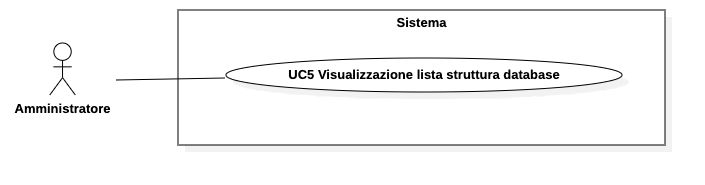
\includegraphics[scale=0.6]{UML_Use_Cases/UC5.png}
\begin{itemize}
	\item \textbf{Descrizione:} l’amministratore visualizza tutte le Strutture \textit{Database} disponibili;
	\item \textbf{Attori:} amministratore;
	\item \textbf{Precondizioni:} 
	\begin{itemize}
		\item L’amministratore ha effettuato il \textit{login} (\hyperref[sec:UC1]{\textbf{UC1}});
		\item L’amministratore si trova nel pannello amministrativo;
	\end{itemize}
	\item \textbf{Postcondizioni:} 
	\begin{itemize}
		\item L'amministratore può vedere nome e descrizione dei \textit{database} presenti;
	\end{itemize}
	\item \textbf{Scenario principale:} 
	\begin{itemize}
		\item Il programma visualizza la lista dei \textit{database} presenti, con la possibilità di modificarli, visualizzarli o eliminarli;
	\end{itemize}
\end{itemize}

\subsection{UC6 - Visualizzazione singola Struttura \textit{Database}}
\label{sec:UC6}
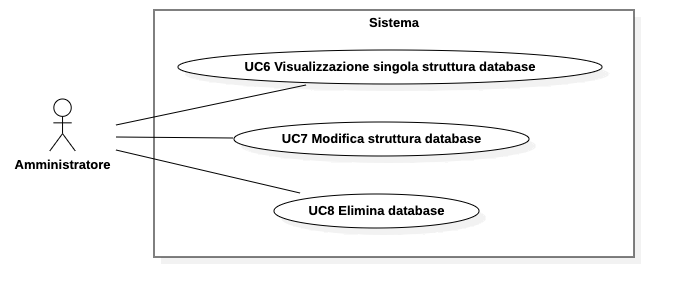
\includegraphics[scale=0.6]{UML_Use_Cases/UC6_7_8.png}
\begin{itemize}
	\item \textbf{Descrizione:} l’amministratore visualizza una Struttura \textit{Database};
	\item \textbf{Attori:} amministratore;
	\item \textbf{Precondizioni:} 
	\begin{itemize}
		\item L’amministratore ha effettuato il \textit{login} (\hyperref[sec:UC1]{\textbf{UC1}});
		\item L’amministratore si trova nel pannello amministrativo;
		\item L'amministratore ha selezionato una Struttura \textit{Database} dalla lista;
	\end{itemize}
	\item \textbf{Postcondizioni:} 
	\begin{itemize}
		\item L'amministratore visualizza il nome della Struttura \textit{Database};
		\item L'amministratore visualizza la descrizione della Struttura \textit{Database};
		\item L'amministratore visualizza la lista delle tabelle della Struttura \textit{Database}  (\hyperref[sec:UC11]{\textbf{UC11}};
	\end{itemize}
	\item \textbf{Scenario principale:} 
	\begin{itemize}
		\item Il programma mostra la lista dei \textit{database} presenti, con la possibilità di modificarli, visualizzarli o eliminarli;
	\end{itemize}
\end{itemize}


\subsection{UC7 - Modifica Struttura \textit{Database}}
\label{sec:UC7}
%\includegraphics[]{diagramma_UML}
\begin{itemize}
	\item \textbf{Descrizione:} l’amministratore modifica la Struttura \textit{Database} selezionata;
	\item \textbf{Attori:} amministratore;
	\item \textbf{Precondizioni:} 
	\begin{itemize}
		\item L’amministratore sta visualizzando una struttura \textit{Database} (\hyperref[sec:UC6]{\textbf{UC6}});
	\end{itemize}
	\item \textbf{Postcondizioni:} 
	\begin{itemize}
		\item Il sistema aggiorna la Struttura \textit{Database};
	\end{itemize}
	\item \textbf{Scenario principale:} 
	\begin{itemize}
		\item L’amministratore modifica il nome del \textit{Database};
		\item Il sistema verifica il nome ricevuto;
	\end{itemize}
	\item \textbf{Estensioni:} nel caso in cui il nuovo nome sia già presente:
	\begin{itemize}
		\item \hyperref[sec:UC4]{\textbf{UC4}} - Errore: nome \textit{Database} già presente.
	\end{itemize}
\end{itemize}

\subsection{UC8 - Elimina \textit{Database}}
\label{sec:UC8}
%\includegraphics[]{diagramma_UML}
\begin{itemize}
	\item \textbf{Descrizione:} l’amministratore elimina la Struttura \textit{Database} selezionata;
	\item \textbf{Attori:} amministratore;
	\item \textbf{Precondizioni:} 
	\begin{itemize}
		\item L’amministratore ha effettuato il \textit{login} (\hyperref[sec:UC1]{\textbf{UC1}});
		\item L’amministratore si trova nel pannello amministrativo;
		\item L’amministratore sta visualizzando la lista dei \textit{database} (\hyperref[sec:UC5]{\textbf{UC5}});
	\end{itemize}
	\item \textbf{Postcondizioni:} 
	\begin{itemize}
		\item La Struttura \textit{Database} selezionata viene eliminata dal sistema;
	\end{itemize}
	\item \textbf{Scenario principale:} 
	\begin{itemize}
		\item L'amministratore seleziona il \textit{database} da eliminare usando il pulsante di eliminazione apposito;
		\item Il sistema visualizza un messaggio per chiedere la conferma dell'eliminazione;
		\item Se l'amministratore conferma l'eliminazione, il \textit{database} e le tabelle collegate verranno rimossi dal sistema e verrà visualizzato un messaggio di avvenuta eliminazione.
	\end{itemize}
\end{itemize}

\subsection{UC9 - Creazione tabella \textit{Database}}
\label{sec:UC9}
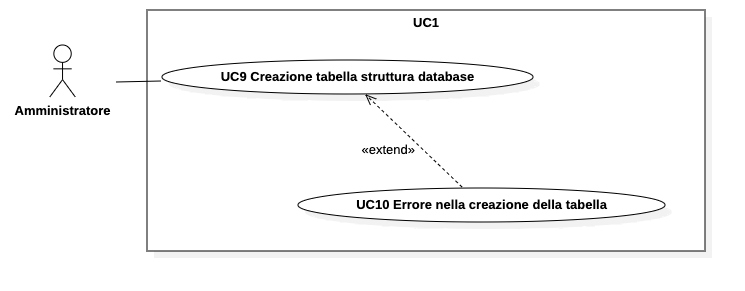
\includegraphics[scale=0.6]{UML_Use_Cases/UC9_10.png}
\begin{itemize}
	\item \textbf{Descrizione:} l’amministratore vuole aggiungere una tabella alla struttura del \textit{database} da interrogare;
	\item \textbf{Attori:} amministratore;
	\item \textbf{Precondizioni:} 
	\begin{itemize}
		\item L’amministratore ha effettuato il \textit{login} (\hyperref[sec:UC1]{\textbf{UC1}});
		\item L’amministratore si trova nel pannello amministrativo;
		\item L’amministratore si trova nella sezione di creazione di una nuova tabella;
	\end{itemize}
	\item \textbf{Postcondizioni:} 
	\begin{itemize}
		\item La tabella viene aggiunta alla struttura del \textit{database};
	\end{itemize}
	\item \textbf{Scenario principale:} 
	\begin{itemize}
		\item L’amministratore inserisce il nome, i sinonimi del nome e la descrizione della tabella;
	\end{itemize}
	\item \textbf{Generalizzazioni:} 
	\begin{itemize}
		\item \hyperref[sec:UC9.1]{\textbf{UC9.1}} - Inserimento nome tabella
		\item \hyperref[sec:UC9.2]{\textbf{UC9.2}} - Inserimento sinonimi tabella
		\item \hyperref[sec:UC9.3]{\textbf{UC9.3}} - Inserimento descrizione tabella
	\end{itemize}
	\item \textbf{Estensioni:} nel caso in cui non vengano inseriti i sinonimi del nome della tabella, o il nome esisti già:
	\begin{itemize}
		\item \hyperref[sec:UC10]{\textbf{UC10}} - Errore nella creazione della tabella
	\end{itemize}
\end{itemize}

\subsubsection{UC9.1 - Inserimento nome tabella}
\label{sec:UC9.1}
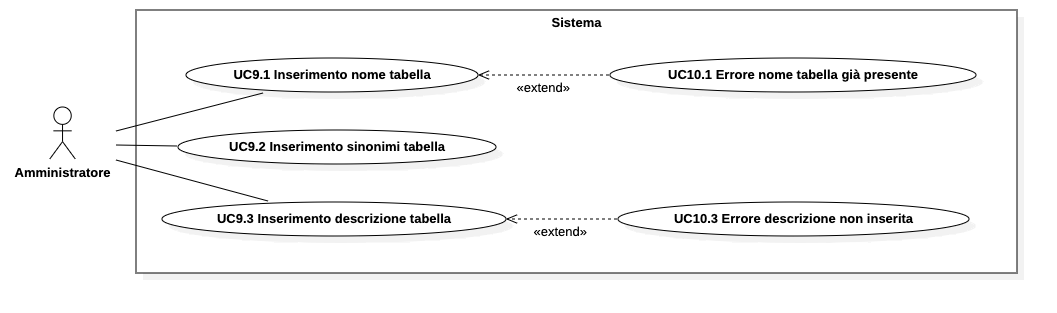
\includegraphics[scale=0.47]{UML_Use_Cases/UC9.1_9.2_9.3_10.1_10.2_10.3.png}
\begin{itemize}
	\item \textbf{Descrizione:} l’amministratore inserisce il nome della tabella da creare;
	\item \textbf{Attori:} amministratore;
	\item \textbf{Precondizioni:} 
	\begin{itemize}
		\item L’amministratore ha effettuato il \textit{login} (\hyperref[sec:UC1]{\textbf{UC1}});
		\item L’amministratore sta creando una nuova tabella (\hyperref[sec:UC9]{\textbf{UC9}});
	\end{itemize}
	\item \textbf{Postcondizioni:} 
	\begin{itemize}
		\item Il nome della tabella viene inserito nel form;
	\end{itemize}
	\item \textbf{Scenario principale:} 
	\begin{itemize}
		\item L’amministratore inserisce il nome della tabella nell'apposito form di creazione;
	\end{itemize}
\end{itemize}

\subsubsection{UC9.2 - Inserimento sinonimi tabella}
\label{sec:UC9.2}
%\includegraphics[]{diagramma_UML}
\begin{itemize}
	\item \textbf{Descrizione:} l’amministratore inserisce i sinonimi associati al nome della tabella da creare;
	\item \textbf{Attori:} amministratore;
	\item \textbf{Precondizioni:} 
	\begin{itemize}
		\item L’amministratore ha effettuato il \textit{login} (\hyperref[sec:UC1]{\textbf{UC1}});
		\item L’amministratore sta creando una nuova tabella (\hyperref[sec:UC9]{\textbf{UC9}});
	\end{itemize}
	\item \textbf{Postcondizioni:} 
	\begin{itemize}
		\item I sinonimi del nome della tabella vengono inseriti nel form;
	\end{itemize}
	\item \textbf{Scenario principale:} 
	\begin{itemize}
		\item L’amministratore inserisce i sinonimi del nome della tabella nell'apposito form di creazione;
	\end{itemize}
\end{itemize}

\subsubsection{UC9.3 - Inserimento descrizione tabella}
\label{sec:UC9.3}
%\includegraphics[]{diagramma_UML}
\begin{itemize}
	\item \textbf{Descrizione:} l’amministratore inserisce la descrizione della tabella da creare;
	\item \textbf{Attori:} amministratore;
	\item \textbf{Precondizioni:} 
	\begin{itemize}
		\item L’amministratore ha effettuato il \textit{login} (\hyperref[sec:UC1]{\textbf{UC1}});
		\item L’amministratore sta creando una nuova tabella (\hyperref[sec:UC9]{\textbf{UC9}});
	\end{itemize}
	\item \textbf{Postcondizioni:} 
	\begin{itemize}
		\item La descrizione della tabella viene inserita nel form;
	\end{itemize}
	\item \textbf{Scenario principale:} 
	\begin{itemize}
		\item L’amministratore inserisce la descrizione della tabella nell'apposito form di creazione;
	\end{itemize}
\end{itemize}

\subsection{UC10 - Errore nella creazione della tabella}
\label{sec:UC10}
%\includegraphics[]{diagramma_UML}
\begin{itemize}
	\item \textbf{Descrizione:} L’amministratore visualizza un errore di creazione della tabella;
	\item \textbf{Attori:} amministratore;
	\item \textbf{Precondizioni:} 
	\begin{itemize}
		\item L’amministratore ha effettuato il \textit{login} (\hyperref[sec:UC1]{\textbf{UC1}});
		\item L’amministratore sta creando una nuova tabella (\hyperref[sec:UC9]{\textbf{UC9}});
	\end{itemize}
	\item \textbf{Postcondizioni:} 
	\begin{itemize}
		\item La tabella non viene creata e il programma visualizza un messaggio di errore;
	\end{itemize}
	\item \textbf{Scenario principale:} 
	\begin{itemize}
		\item L’amministratore inserisce il nome della tabella nel form di creazione (\hyperref[sec:UC9.1]{\textbf{UC9.1}});
		\item L’amministratore inserisce i sinonimi del nome della tabella nel form di creazione (\hyperref[sec:UC9.2]{\textbf{UC9.2}});
		\item L’amministratore inserisce la descrizione della tabella nel form di creazione (\hyperref[sec:UC9.3]{\textbf{UC9.3}});
		\item Il sistema verifica che non esista già una tabella con lo stesso nome e che vengano inseriti sinonimi e descrizione della tabella;
		\item Il sistema visualizza il messaggio di errore opportuno.
	\end{itemize}
\end{itemize}

\subsubsection{UC10.1 - Errore nome tabella già presente}
\label{sec:UC10.1}
%\includegraphics[]{diagramma_UML}
\begin{itemize}
	\item \textbf{Descrizione:} L’amministratore visualizza un errore relativo al nome della tabella;
	\item \textbf{Attori:} amministratore;
	\item \textbf{Precondizioni:} 
	\begin{itemize}
		\item L’amministratore ha effettuato il \textit{login} (\hyperref[sec:UC1]{\textbf{UC1}});
		\item L’amministratore sta creando una nuova tabella (\hyperref[sec:UC9]{\textbf{UC9}});
	\end{itemize}
	\item \textbf{Postcondizioni:} 
	\begin{itemize}
		\item La tabella non viene creata e il programma visualizza un messaggio di errore;
	\end{itemize}
	\item \textbf{Scenario principale:} 
	\begin{itemize}
		\item Il sistema verifica che non esista già una tabella con lo stesso nome;
		\item Il sistema visualizza il messaggio di errore per il nome inserito.
	\end{itemize}
\end{itemize}

\subsubsection{UC10.2 - Errore sinonimi non inseriti}
\label{sec:UC10.2}
%\includegraphics[]{diagramma_UML}
\begin{itemize}
	\item \textbf{Descrizione:} L’amministratore visualizza un errore relativo ai sinonimi del nome della tabella;
	\item \textbf{Attori:} amministratore;
	\item \textbf{Precondizioni:} 
	\begin{itemize}
		\item L’amministratore ha effettuato il \textit{login} (\hyperref[sec:UC1]{\textbf{UC1}});
		\item L’amministratore sta creando una nuova tabella (\hyperref[sec:UC9]{\textbf{UC9}});
	\end{itemize}
	\item \textbf{Postcondizioni:} 
	\begin{itemize}
		\item La tabella non viene creata e il programma visualizza un messaggio di errore;
	\end{itemize}
	\item \textbf{Scenario principale:} 
	\begin{itemize}
		\item Il sistema verifica che il campo relativo ai sinonimi del nome della tabella non sia vuoto;
		\item Il sistema visualizza il messaggio di errore per il campo sinonimi vuoto.
	\end{itemize}
\end{itemize}

\subsubsection{UC10.3 - Errore descrizione non inserita}
\label{sec:UC10.3}
%\includegraphics[]{diagramma_UML}
\begin{itemize}
	\item \textbf{Descrizione:} L’amministratore visualizza un errore relativo alla descrizione della tabella;
	\item \textbf{Attori:} amministratore;
	\item \textbf{Precondizioni:} 
	\begin{itemize}
		\item L’amministratore ha effettuato il \textit{login} (\hyperref[sec:UC1]{\textbf{UC1}});
		\item L’amministratore sta creando una nuova tabella (\hyperref[sec:UC9]{\textbf{UC9}});
	\end{itemize}
	\item \textbf{Postcondizioni:} 
	\begin{itemize}
		\item La tabella non viene creata e il programma visualizza un messaggio di errore;
	\end{itemize}
	\item \textbf{Scenario principale:} 
	\begin{itemize}
		\item Il sistema verifica che il campo relativo ai sinonimi del nome della tabella non sia vuoto;
		\item Il sistema visualizza il messaggio di errore per il campo descrizione vuoto.
	\end{itemize}
\end{itemize}

\subsection{UC11 - Visualizzazione lista delle tabelle nella Struttura \textit{Database}}
\label{sec:UC11}
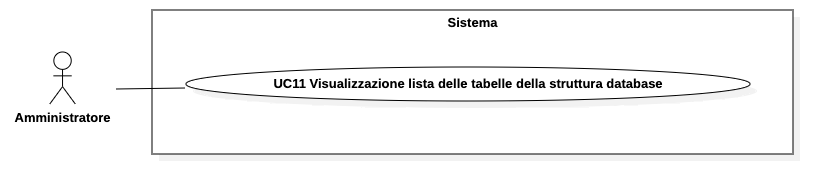
\includegraphics[scale=0.6]{UML_Use_Cases/UC11.png}
\begin{itemize}
	\item \textbf{Descrizione:} l’amministratore visualizza tutte le tabelle della Struttura \textit{Database} selezionata;
	\item \textbf{Attori:} amministratore;
	\item \textbf{Precondizioni:} 
	\begin{itemize}
		\item L’amministratore ha effettuato il \textit{login} (\hyperref[sec:UC1]{\textbf{UC1}});
		\item L’amministratore si trova nel pannello amministrativo;
		\item L'amministratore ha selezionato una Struttura \textit{Database} dalla lista;
	\end{itemize}
	\item \textbf{Postcondizioni:} 
	\begin{itemize}
		\item L'amministratore può vedere il nome delle tabelle presenti;
	\end{itemize}
	\item \textbf{Scenario principale:} 
	\begin{itemize}
		\item Il programma visualizza la lista delle tabelle presenti, con la possibilità di modificarle, visualizzarle o eliminarle;
	\end{itemize}
\end{itemize}

\subsection{UC12 - Visualizzazione della singola tabella}
\label{sec:UC12}
%\includegraphics[]{diagramma_UML}
\begin{itemize}
	\item \textbf{Descrizione:} l’amministratore visualizza la tabella della Struttura \textit{Database} selezionata;
	\item \textbf{Attori:} amministratore;
	\item \textbf{Precondizioni:} 
	\begin{itemize}
		\item L'amministratore ha visualizzato la lista delle tabelle della Struttura \textit{Database} (\hyperref[sec:UC11]{\textbf{UC11}});
		\item L'amministratore ha selezionato una tabella dalla lista;
	\end{itemize}
	\item \textbf{Postcondizioni:} 
	\begin{itemize}
		\item L'amministratore può vedere nome, descrizione e sinonimi della tabella selezionata;
		\item L'amministratore può visualizzare i campi della tabella selezionata;
	\end{itemize}
	\item \textbf{Scenario principale:} 
	\begin{itemize}
		\item Il programma visualizza i campi della tabella selezionata;
	\end{itemize}
\end{itemize}

\subsection{UC13 - Modifica della tabella}
\label{sec:UC13}
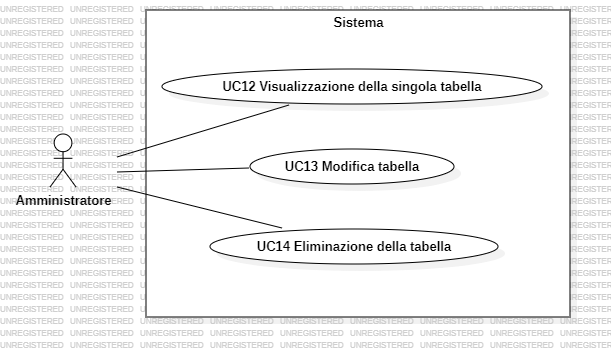
\includegraphics[scale=0.6]{UML_Use_Cases/UC12_13_14.png}
\begin{itemize}
	\item \textbf{Descrizione:} l’amministratore vuole modificare una tabella del \textit{database} selezionato e da interrogare;
	\item \textbf{Attori:} amministratore;
	\item \textbf{Precondizioni:} 
	\begin{itemize}
		\item L’amministratore ha effettuato il \textit{login} (\hyperref[sec:UC1]{\textbf{UC1}});
		\item L’amministratore si trova nel pannello amministrativo;
		\item L’amministratore si trova nella sezione di modifica di una tabella;
	\end{itemize}
	\item \textbf{Postcondizioni:} 
	\begin{itemize}
		\item La tabella selezionata viene modificata;
	\end{itemize}
	\item \textbf{Scenario principale:} 
	\begin{itemize}
		\item L’amministratore modifica il nome, i sinonimi del nome e la descrizione della tabella;
	\end{itemize}
	\item \textbf{Estensioni:} nel caso in cui non vengano rimossi completamente i sinonimi del nome della tabella, o il nome modificato è già presente:
	\begin{itemize}
		\item \hyperref[sec:UC10]{\textbf{UC10}} - Errore nella creazione della tabella
	\end{itemize}
\end{itemize}

\subsection{UC14 - Eliminazione della tabella}
\label{sec:UC14}
%\includegraphics[]{diagramma_UML}
\begin{itemize}
	\item \textbf{Descrizione:} l’amministratore elimina la tabella selezionata;
	\item \textbf{Attori:} amministratore;
	\item \textbf{Precondizioni:} 
	\begin{itemize}
		\item L’amministratore ha effettuato il \textit{login} (\hyperref[sec:UC1]{\textbf{UC1}});
		\item L’amministratore si trova nel pannello amministrativo;
		\item L’amministratore sta visualizzando la lista delle tabelle (\hyperref[sec:UC11]{\textbf{UC11}});
	\end{itemize}
	\item \textbf{Postcondizioni:} 
	\begin{itemize}
		\item La Struttura \textit{Database} selezionata viene eliminata dal sistema;
	\end{itemize}
	\item \textbf{Scenario principale:} 
	\begin{itemize}
		\item L'amministratore seleziona la tabella da eliminare usando il pulsante di eliminazione apposito;
		\item Il sistema visualizza un messaggio per chiedere la conferma dell'eliminazione;
		\item Se l'amministratore conferma l'eliminazione, la tabella e i suoi campi verranno rimossi dal sistema e verrà visualizzato un messaggio di avvenuta eliminazione.
	\end{itemize}
\end{itemize}

\subsection{UC15 - Creazione campo tabella}
\label{sec:UC15}
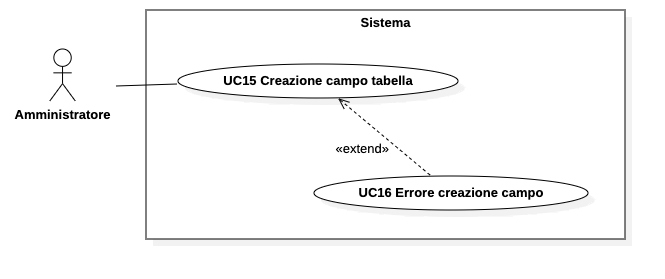
\includegraphics[scale=0.6]{UML_Use_Cases/UC15_16.png}
\begin{itemize}
	\item \textbf{Descrizione:} l’amministratore vuole aggiungere un campo alla tabella selezionata;
	\item \textbf{Attori:} amministratore;
	\item \textbf{Precondizioni:} 
	\begin{itemize}
		\item L’amministratore ha effettuato il \textit{login} (\hyperref[sec:UC1]{\textbf{UC1}});
		\item L’amministratore si trova nel pannello amministrativo;
		\item L’amministratore si trova nella sezione di visualizzazione di una tabella (\hyperref[sec:UC12]{\textbf{UC12}});
		\item L’amministratore sta inserendo i campi che compongono la tabella;
	\end{itemize}
	\item \textbf{Postcondizioni:} 
	\begin{itemize}
		\item I campi vengono aggiunti alla tabella;
	\end{itemize}
	\item \textbf{Scenario principale:} 
	\begin{itemize}
		\item L’amministratore inserisce il nome del campo \hyperref[sec:UC15.1]{\textbf{UC15.1}};
		\item L'amministratore seleziona il tipo del campo \hyperref[sec:UC15.2]{\textbf{UC15.2}};
		\item L'amministratore inserisce i sinonimi del campo \hyperref[sec:UC15.3]{\textbf{UC15.3}};
	\end{itemize}
	\item \textbf{Estensioni:} nel caso in cui il nome inserito sia già esistente o non sia stato selezionato il tipo o inseriti i sinonimi:
	\begin{itemize}
		\item \hyperref[sec:UC16]{\textbf{UC16}} - Errore creazione campo
	\end{itemize}
\end{itemize}

\subsubsection{UC15.1 - Inserimento nome campo}
\label{sec:UC15.1}
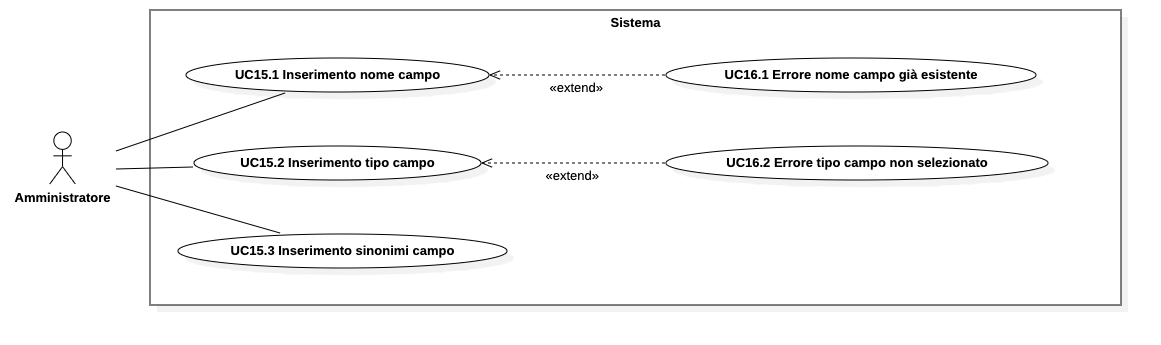
\includegraphics[scale=0.45]{UML_Use_Cases/UC15.1_15.2_15.3_16.1_16.2_16.3.png}
\begin{itemize}
	\item \textbf{Descrizione:} l’amministratore vuole inserire il nome del campo da inserire nella tabella;
	\item \textbf{Attori:} amministratore;
	\item \textbf{Precondizioni:} 
	\begin{itemize}
		\item L’amministratore ha effettuato il \textit{login} (\hyperref[sec:UC1]{\textbf{UC1}});
		\item L’amministratore si trova nel pannello amministrativo;
		\item L’amministratore si trova nella sezione di visualizzazione di una tabella (\hyperref[sec:UC12]{\textbf{UC12}});
		\item L’amministratore sta inserendo i campi che compongono la tabella;
	\end{itemize}
	\item \textbf{Postcondizioni:} 
	\begin{itemize}
		\item Il nome del campo viene inserito;
	\end{itemize}
	\item \textbf{Scenario principale:} 
	\begin{itemize}
		\item L’amministratore inserisce il nome del campo nella casella di testo dedicata;
	\end{itemize}
	\item \textbf{Estensioni:} nel caso in cui il nome inserito sia già esistente:
	\begin{itemize}
		\item \hyperref[sec:UC16.1]{\textbf{UC16.1}} - Errore nome campo già esistente
	\end{itemize}
\end{itemize}

\subsubsection{UC15.2 - Inserimento tipo campo}
\label{sec:UC15.2}
%\includegraphics[]{diagramma_UML}
\begin{itemize}
	\item \textbf{Descrizione:} l’amministratore vuole selezionare il tipo del campo da inserire nella tabella;
	\item \textbf{Attori:} amministratore;
	\item \textbf{Precondizioni:} 
	\begin{itemize}
		\item L’amministratore ha effettuato il \textit{login} (\hyperref[sec:UC1]{\textbf{UC1}});
		\item L’amministratore si trova nel pannello amministrativo;
		\item L’amministratore si trova nella sezione di visualizzazione di una tabella (\hyperref[sec:UC12]{\textbf{UC12}}) ;
		\item L’amministratore sta inserendo i campi che compongono la tabella;
	\end{itemize}
	\item \textbf{Postcondizioni:} 
	\begin{itemize}
		\item Il tipo del campo viene selezionato;
	\end{itemize}
	\item \textbf{Scenario principale:} 
	\begin{itemize}
		\item L’amministratore sceglie il tipo di campo, selezionandolo dalle scelte possibili;
	\end{itemize}
	\item \textbf{Estensioni:} nel caso in cui il tipo non venga selezionato:
	\begin{itemize}
		\item \hyperref[sec:UC16.2]{\textbf{UC16.2}} - Errore tipo campo non selezionato
	\end{itemize}
\end{itemize}

\subsubsection{UC15.3 - Inserimento sinonimi campo}
\label{sec:UC15.3}
%\includegraphics[]{diagramma_UML}
\begin{itemize}
	\item \textbf{Descrizione:} l’amministratore vuole inserire i sinonimi del campo da inserire nella tabella;
	\item \textbf{Attori:} amministratore;
	\item \textbf{Precondizioni:} 
	\begin{itemize}
		\item L’amministratore ha effettuato il \textit{login} (\hyperref[sec:UC1]{\textbf{UC1}});
		\item L’amministratore si trova nel pannello amministrativo;
		\item L’amministratore si trova nella sezione di visualizzazione di una tabella (\hyperref[sec:UC12]{\textbf{UC12}} ;
		\item L’amministratore sta inserendo i campi che compongono la tabella;
	\end{itemize}
	\item \textbf{Postcondizioni:} 
	\begin{itemize}
		\item I sinonimi del nome del campo vengono inseriti;
	\end{itemize}
	\item \textbf{Scenario principale:} 
	\begin{itemize}
		\item L’amministratore inserisce i sinonimi del nome del campo nella casella di testo dedicata;
	\end{itemize}
	\item \textbf{Estensioni:} nel caso in cui i sinonimi non vengano inseriti:
	\begin{itemize}
		\item \hyperref[sec:UC16.3]{\textbf{UC16.3}} - Errore mancato inserimento sinonimi campo
	\end{itemize}
\end{itemize}

\subsection{UC16 - Errore creazione campo}
\label{sec:UC16}
%\includegraphics[]{diagramma_UML}
\begin{itemize}
	\item \textbf{Descrizione:} L’amministratore visualizza un errore di creazione del campo;
	\item \textbf{Attori:} amministratore;
	\item \textbf{Precondizioni:} 
	\begin{itemize}
		\item L’amministratore ha effettuato il \textit{login} (\hyperref[sec:UC1]{\textbf{UC1}});
		\item L’amministratore si trova nel pannello amministrativo;
		\item L’amministratore si trova nella sezione di visualizzazione di una tabella (\hyperref[sec:UC12]{\textbf{UC12}} ;
		\item L’amministratore sta creando un nuovo campo (\hyperref[sec:UC15]{\textbf{UC15}});
	\end{itemize}
	\item \textbf{Postcondizioni:} 
	\begin{itemize}
		\item Il campo non viene creato e il programma visualizza un messaggio di errore;
	\end{itemize}
	\item \textbf{Scenario principale:} 
	\begin{itemize}
		\item L’amministratore inserisce il nome del campo nel form di creazione (\hyperref[sec:UC15.1]{\textbf{UC15.1}});
		\item L’amministratore seleziona il tipo del campo nel form di creazione (\hyperref[sec:UC15.2]{\textbf{UC15.2}});
		\item L’amministratore inserisce i sinonimi del nome campo nel form di creazione (\hyperref[sec:UC15.3]{\textbf{UC15.3}});
		\item Il sistema verifica che non esista già una tabella con lo stesso nome, che venga selezionato il tipo e che vengano inseriti i sinonimi del campo;
		\item Il sistema visualizza il messaggio di errore opportuno.
	\end{itemize}
\end{itemize}

\subsubsection{UC16.1 - Errore nome campo già esistente}
\label{sec:UC16.1}
%\includegraphics[]{diagramma_UML}
\begin{itemize}
	\item \textbf{Descrizione:} L’amministratore visualizza un errore relativo al nome del campo;
	\item \textbf{Attori:} amministratore;
	\item \textbf{Precondizioni:} 
	\begin{itemize}
		\item L’amministratore ha effettuato il \textit{login} (\hyperref[sec:UC1]{\textbf{UC1}});
		\item L’amministratore si trova nel pannello amministrativo;
		\item L’amministratore si trova nella sezione di visualizzazione di una tabella (\hyperref[sec:UC12]{\textbf{UC12}} ;
		\item L’amministratore sta creando un nuovo campo (\hyperref[sec:UC15]{\textbf{UC15}});
	\end{itemize}
	\item \textbf{Postcondizioni:} 
	\begin{itemize}
		\item Il campo non viene creato e il programma visualizza un messaggio di errore;
	\end{itemize}
	\item \textbf{Scenario principale:} 
	\begin{itemize}
		\item Il sistema verifica che non esista già un campo con lo stesso nome;
		\item Il sistema visualizza il messaggio di errore per il nome inserito.
	\end{itemize}
\end{itemize}

\subsubsection{UC16.2 - Errore tipo campo non selezionato}
\label{sec:UC16.2}
%\includegraphics[]{diagramma_UML}
\begin{itemize}
	\item \textbf{Descrizione:} L’amministratore visualizza un errore relativo al tipo del campo;
	\item \textbf{Attori:} amministratore;
	\item \textbf{Precondizioni:} 
	\begin{itemize}
		\item L’amministratore ha effettuato il \textit{login} (\hyperref[sec:UC1]{\textbf{UC1}});
		\item L’amministratore si trova nel pannello amministrativo;
		\item L’amministratore si trova nella sezione di visualizzazione di una tabella (\hyperref[sec:UC12]{\textbf{UC12}} ;
		\item L’amministratore sta creando un nuovo campo (\hyperref[sec:UC15]{\textbf{UC15}});
	\end{itemize}
	\item \textbf{Postcondizioni:} 
	\begin{itemize}
		\item Il campo non viene creato e il programma visualizza un messaggio di errore;
	\end{itemize}
	\item \textbf{Scenario principale:} 
	\begin{itemize}
		\item Il sistema verifica che sia stato selezionato un tipo tra quelli disponibili per il campo;
		\item Il sistema visualizza il messaggio di errore per il tipo del campo.
	\end{itemize}
\end{itemize}

\subsubsection{UC16.3 - Errore mancato inserimento sinonimi campo}
\label{sec:UC16.3}
%\includegraphics[]{diagramma_UML}
\begin{itemize}
	\item \textbf{Descrizione:} L’amministratore visualizza un errore relativo ai sinonimi del nome del campo;
	\item \textbf{Attori:} amministratore;
	\item \textbf{Precondizioni:} 
	\begin{itemize}
		\item L’amministratore ha effettuato il \textit{login} (\hyperref[sec:UC1]{\textbf{UC1}});
		\item L’amministratore si trova nel pannello amministrativo;
		\item L’amministratore si trova nella sezione di visualizzazione di una tabella (\hyperref[sec:UC12]{\textbf{UC12}} ;
		\item L’amministratore sta creando un nuovo campo (\hyperref[sec:UC15]{\textbf{UC15}});
	\end{itemize}
	\item \textbf{Postcondizioni:} 
	\begin{itemize}
		\item Il campo non viene creato e il programma visualizza un messaggio di errore;
	\end{itemize}
	\item \textbf{Scenario principale:} 
	\begin{itemize}
		\item Il sistema verifica che siano stati inseriti dei sinonimi per il nome del campo;
		\item Il sistema visualizza il messaggio di errore per i sinonimi.
	\end{itemize}
\end{itemize}

\subsection{UC17 - Visualizzazione lista dei campi della tabella}
\label{sec:UC17}
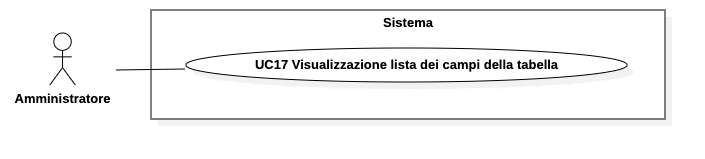
\includegraphics[scale=0.6]{UML_Use_Cases/UC17.png}
\begin{itemize}
	\item \textbf{Descrizione:} l’amministratore visualizza tutti i campi della tabella selezionata;
	\item \textbf{Attori:} amministratore;
	\item \textbf{Precondizioni:} 
	\begin{itemize}
		\item L’amministratore ha effettuato il \textit{login} (\hyperref[sec:UC1]{\textbf{UC1}});
		\item L’amministratore si trova nella sezione di visualizzazione di una tabella (\hyperref[sec:UC12]{\textbf{UC12}} ;
		\item L’amministratore si trova nel pannello amministrativo;
	\end{itemize}
	\item \textbf{Postcondizioni:} 
	\begin{itemize}
		\item L'amministratore può vedere nome, tipo e sinonimi dei campi presenti;
	\end{itemize}
	\item \textbf{Scenario principale:} 
	\begin{itemize}
		\item Il programma visualizza la lista dei campi presenti, con la possibilità di modificarli, visualizzarli o eliminarli;
	\end{itemize}
\end{itemize}

\subsection{UC18 - Visualizzazione singolo campo tabella}
\label{sec:UC18}
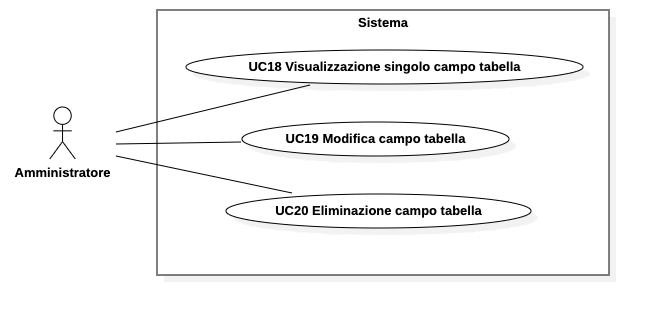
\includegraphics[scale=0.6]{UML_Use_Cases/UC18_19_20.png}
\begin{itemize}
	\item \textbf{Descrizione:} l’amministratore visualizza tutti i campi della tabella selezionata;
	\item \textbf{Attori:} amministratore;
	\item \textbf{Precondizioni:} 
	\begin{itemize}
		\item L’amministratore ha effettuato il \textit{login} (\hyperref[sec:UC1]{\textbf{UC1}});
		\item L’amministratore si trova nella sezione di visualizzazione di una tabella (\hyperref[sec:UC12]{\textbf{UC12}});
		\item L’amministratore si trova nel pannello amministrativo;
		\item L'amministratore ha selezionato un campo di una tabella;
	\end{itemize}
	\item \textbf{Postcondizioni:} 
	\begin{itemize}
		\item L'amministratore può vedere nome, tipo e sinonimi del campo selezionatoi;
	\end{itemize}
	\item \textbf{Scenario principale:} 
	\begin{itemize}
		\item Il programma visualizza la lista dei campi presenti, con la possibilità di modificarli, visualizzarli o eliminarli;
	\end{itemize}
\end{itemize}

\subsection{UC19 - Modifica campo tabella}
\label{sec:UC19}
%\includegraphics[]{diagramma_UML}
\begin{itemize}
	\item \textbf{Descrizione:} l’amministratore vuole modificare un campo alla tabella selezionata;
	\item \textbf{Attori:} amministratore;
	\item \textbf{Precondizioni:} 
	\begin{itemize}
		\item L’amministratore ha effettuato il \textit{login} (\hyperref[sec:UC1]{\textbf{UC1}});
		\item L’amministratore si trova nel pannello amministrativo;
		\item L’amministratore si trova nella sezione di visualizzazione di una tabella (\hyperref[sec:UC12]{\textbf{UC12}});
		\item L’amministratore sta modificando i campi che compongono la tabella;
	\end{itemize}
	\item \textbf{Postcondizioni:} 
	\begin{itemize}
		\item I campi della tabella vengono modificati;
	\end{itemize}
	\item \textbf{Scenario principale:} 
	\begin{itemize}
		\item L’amministratore inserisce il nome del campo \hyperref[sec:UC15.1]{\textbf{UC15.1}};
		\item L'amministratore seleziona il tipo del campo \hyperref[sec:UC15.2]{\textbf{UC15.2}};
		\item L'amministratore inserisce i sinonimi del campo \hyperref[sec:UC15.3]{\textbf{UC15.3}};
	\end{itemize}

		\item \textbf{Estensioni:} nel caso in cui il nome inserito sia già esistente o non sia stato selezionato il tipo o inseriti i sinonimi:
		\begin{itemize}
			\item (\hyperref[sec:UC16]{\textbf{UC16}}) - Errore creazione campo
	\end{itemize}
\end{itemize}


\subsection{UC20 - Eliminazione campo tabella}
\label{sec:UC20}
%\includegraphics[]{diagramma_UML}
\begin{itemize}
	\item \textbf{Descrizione:} l’amministratore elimina il campo selezionato;
	\item \textbf{Attori:} amministratore;
	\item \textbf{Precondizioni:} 
	\begin{itemize}
		\item L’amministratore ha effettuato il \textit{login} (\hyperref[sec:UC1]{\textbf{UC1}});
		\item L’amministratore si trova nel pannello amministrativo;
		\item L’amministratore sta visualizzando la lista dei campi (\hyperref[sec:UC15]{\textbf{UC15}});
	\end{itemize}
	\item \textbf{Postcondizioni:} 
	\begin{itemize}
		\item Il campo selezionato viene eliminato dal sistema;
	\end{itemize}
	\item \textbf{Scenario principale:} 
	\begin{itemize}
		\item L'amministratore seleziona il campo da eliminare;
		\item Il sistema visualizza un messaggio per chiedere la conferma dell'eliminazione;
		\item Se l'amministrazione conferma l'eliminazione, il campo verrà rimosso dal sistema e verrà visualizzato un messaggio di avvenuta eliminazione.
	\end{itemize}
\end{itemize}

\subsection{UC21 - Caricamento struttura \textit{Database} tramite file}
\label{sec:UC21}
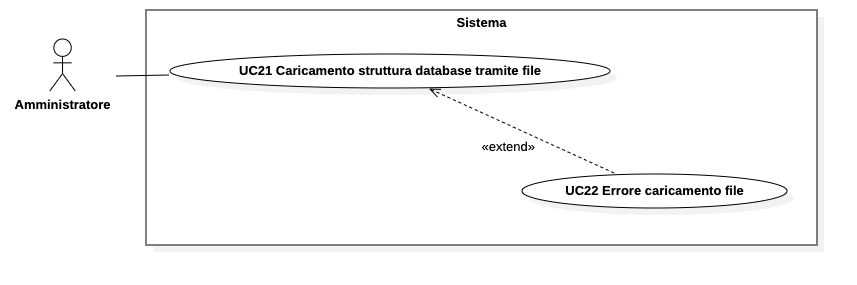
\includegraphics[scale=0.6]{UML_Use_Cases/UC21_22.png}
\begin{itemize}
	\item \textbf{Descrizione:} l’amministratore vuole caricare un file che descrive una Struttura \textit{Database};
	\item \textbf{Attori:} amministratore;
	\item \textbf{Precondizioni:} 
	\begin{itemize}
		\item L’amministratore ha effettuato il \textit{login} (\hyperref[sec:UC1]{\textbf{UC1}});
		\item L’amministratore si trova nel pannello amministrativo;
	\end{itemize}
	\item \textbf{Postcondizioni:} 
	\begin{itemize}
		\item La Struttura \textit{Database} viene caricata correttamente nel sistema;
	\end{itemize}
	\item \textbf{Scenario principale:} 
	\begin{itemize}
		\item L'amministrazione inserisce il file della Struttura \textit{Database};
	\end{itemize}
	\item \textbf{Estensioni:} nel caso il file non sia corretto:
	\begin{itemize}
		\item \hyperref[sec:UC22]{\textbf{UC22}} - Errore caricamento file
	\end{itemize}
\end{itemize}

\subsection{UC22 - Errore caricamento file}
\label{sec:UC22}
\begin{itemize}
	\item \textbf{Descrizione:} L’amministratore visualizza un errore di caricamento del file;
	\item \textbf{Attori:} amministratore;
	\item \textbf{Precondizioni:} 
	\begin{itemize}
		\item L’amministratore ha effettuato il \textit{login} (\hyperref[sec:UC1]{\textbf{UC1}});
		\item L’amministratore si trova nel pannello amministrativo;
		\item L’amministratore sta caricando un file Struttura del \textit{Database} (\hyperref[sec:UC21]{\textbf{UC21}});
	\end{itemize}
	\item \textbf{Postcondizioni:} 
	\begin{itemize}
		\item La Struttura \textit{Database} non viene caricata e salvata, il programma visualizza un messaggio di errore;
	\end{itemize}
	\item \textbf{Scenario principale:} 
	\begin{itemize}
		\item Il sistema verifica che il formato del file sia corretto;
		\item Il sistema mostra un messaggio di errore se il formato non è corretto;
	\end{itemize}
\end{itemize}


\subsection{UC23 - \textit{Logout}}
\label{sec:UC23}
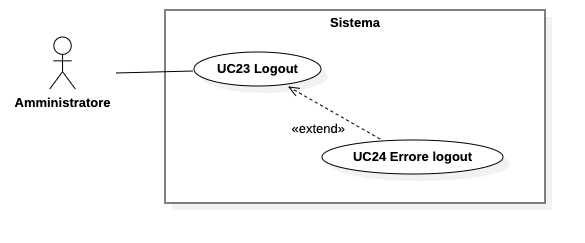
\includegraphics[scale=0.6]{UML_Use_Cases/UC23_24.png}
\begin{itemize}
	\item \textbf{Descrizione:} l'amministratore vuole fare il \textit{logout} dall'area amministrativa; 
	\item \textbf{Attori:} amministratore;
	\item \textbf{Precondizioni:} 
	\begin{itemize}
		\item L’amministratore ha effettuato il \textit{login} (\hyperref[sec:UC1]{\textbf{UC1}});
	\end{itemize}
	\item \textbf{Postcondizioni:} 
	\begin{itemize}
		\item Viene visualizzata la pagina iniziale;
	\end{itemize}
	\item \textbf{Scenario principale:} 
	\begin{itemize}
		\item L’amministratore clicca il pulsante di \textit{logout};
		\item L’amministratore viene reindirizzato alla pagina iniziale.
	\end{itemize}
	\item \textbf{Estensioni:} nel caso in cui l'utente non fosse loggato:
	\begin{itemize}
		\item Viene visualizzato un errore - \hyperref[sec:UC24]{\textbf{UC24}}.
	\end{itemize}
\end{itemize}

\subsection{UC24 - Errore \textit{logout}}
\label{sec:UC24}
\begin{itemize}
	\item \textbf{Descrizione:} L’amministratore visualizza un errore di \textit{logout};
	\item \textbf{Attori:} amministratore;
	\item \textbf{Precondizioni:} 
	\begin{itemize}
		\item L’amministratore sta tentando di fare il \textit{logout} (\hyperref[sec:UC21]{\textbf{UC21}});
		\item La sessione corrente dell'amministratore non è presente;
	\end{itemize}
	\item \textbf{Postcondizioni:} 
	\begin{itemize}
		\item L'amministratore viene reindirizzato alla pagina iniziale, il programma visualizza un messaggio di errore;
	\end{itemize}
	\item \textbf{Scenario principale:} 
	\begin{itemize}
		\item Il sistema verifica la presenza della sessione di \textit{login};
		\item Il sistema mostra un messaggio di errore se la sessione non è presente;
		\item L'amministratore viene riportato alla pagina iniziale.
	\end{itemize}
\end{itemize}

\subsection{UC25 - Selezione Struttura \textit{Database} da interrogare}
\label{sec:UC25}
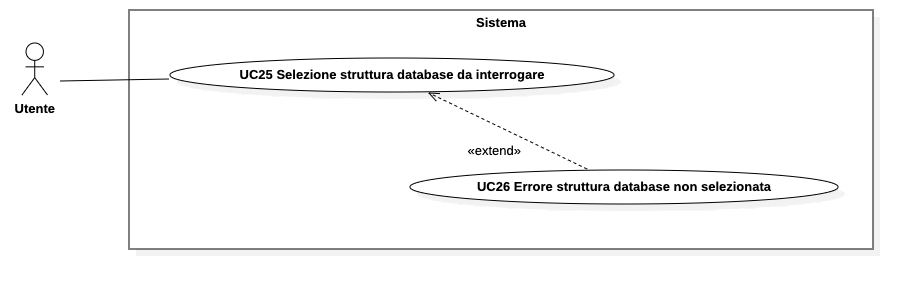
\includegraphics[scale=0.55]{UML_Use_Cases/UC25_26.png}
\begin{itemize}
	\item \textbf{Descrizione:} l’utente seleziona la Struttura \textit{Database} che vuole interrogare da una lista;
	\item \textbf{Attori:} utente;
	\item \textbf{Precondizioni:}
	\begin{itemize}
		\item Sono presenti una o più Strutture \textit{Database} da poter selezionare;
	\end{itemize}
	\item \textbf{Postcondizioni:}
	\begin{itemize}
		\item L’utente ha selezionato una Struttura \textit{Database};
	\end{itemize}
	\item \textbf{Scenario principale:}
	\begin{itemize}
		\item L’utente ha il programma aperto;
		\item L’utente seleziona uno dei \textit{database} presenti nella lista.
	\end{itemize}
	\item \textbf{Estensioni:} In caso l'utente non selezioni una Strttura \textit{Database};
	\begin{itemize}
		\item Errore Struttura \textit{Database} non selezionata (\hyperref[sec:UC26]{\textbf{UC26}});
	\end{itemize}
\end{itemize}

\subsection{UC26 - Errore Struttura \textit{Database} non selezionata}
\label{sec:UC26}
\begin{itemize}
	\item \textbf{Descrizione:} l’utente non ha selezionato una Struttura \textit{Database};
	\item \textbf{Attori:} utente;
	\item \textbf{Precondizioni:}
	\begin{itemize}
		\item Sono presenti una o più Strutture \textit{Database} da poter selezionare;
	\end{itemize}
	\item \textbf{Postcondizioni:}
	\begin{itemize}
		\item L’utente visualizza un messaggio di errore;
	\end{itemize}
	\item \textbf{Scenario principale:}
	\begin{itemize}
		\item Il sistema non riceve una Struttura \textit{Database};
		\item Il sistema mostra un errore;
	\end{itemize}
\end{itemize}

\subsection{UC27 - Inserimento frase in linguaggio naturale}
\label{sec:UC27}
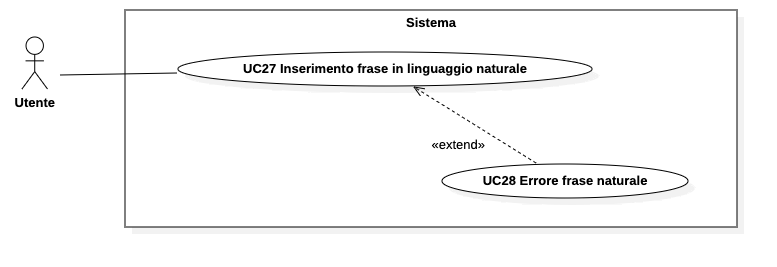
\includegraphics[scale=0.6]{UML_Use_Cases/UC27_28.png}
\begin{itemize}
	\item \textbf{Descrizione:} L’utente scrive una frase in linguaggio naturale;
	\item \textbf{Attori:} utente;
	\item \textbf{Precondizioni:} 
	\begin{itemize}
		\item L’utente ha selezionato un file di struttura \textit{Database} (\hyperref[sec:UC25]{\textbf{UC25}});
	\end{itemize}
	\item \textbf{Postcondizioni:} 
	\begin{itemize}
		\item L’utente riceve un \textit{prompt} per la creazione della \textit{query} richiesta (\hyperref[sec:UC29]{\textbf{UC29}});
	\end{itemize}
	\item \textbf{Scenario principale:} 
	\begin{itemize}
		\item L’utente ha il programma aperto;
		\item L’utente seleziona la casella di testo;
		\item L’utente scrive la frase per interrogare il \textit{database};
		\item L’utente clicca il pulsante apposito per ottenere il \textit{prompt}.
	\end{itemize}
	\item \textbf{Estensioni:} nel caso in cui venga inserita una frase non inerente al \textit{database}, o non comprensibile:
	\begin{itemize}
		\item Viene visualizzato un errore - \hyperref[sec:UC28]{\textbf{UC28}}.
	\end{itemize}
\end{itemize}

\subsection{UC28 - Errore frase naturale}
\label{sec:UC28}
\begin{itemize}
	\item \textbf{Descrizione:} L’utente visualizza un errore inerente alla frase inserita;
	\item \textbf{Attori:} utente;
	\item \textbf{Precondizioni:} 
	\begin{itemize}
		\item L’utente ha selezionato un file di struttura \textit{Database} (\hyperref[sec:UC25]{\textbf{UC25}});
		\item L'utente ha inserito una frase in linguaggio naturale (\hyperref[sec:UC27]{\textbf{UC27}});
	\end{itemize}
	\item \textbf{Postcondizioni:} 
	\begin{itemize}
		\item L’utente visualizza un messaggio di errore;
	\end{itemize}
	\item \textbf{Scenario principale:} 
	\begin{itemize}
		\item Il sistema verifica la frase ricevuta;
		\item Il sistema non riesce ad elaborare la frase;
		\item Il sistema visualizza un messaggio di errore.
	\end{itemize}
\end{itemize}

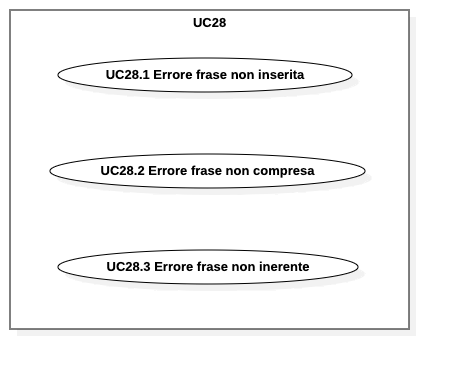
\includegraphics[scale=0.6]{UML_Use_Cases/UC28.1_28.2_28.3.png}

\subsubsection{UC28.1 - Errore frase non inserita}
\label{sec:UC28.1}
%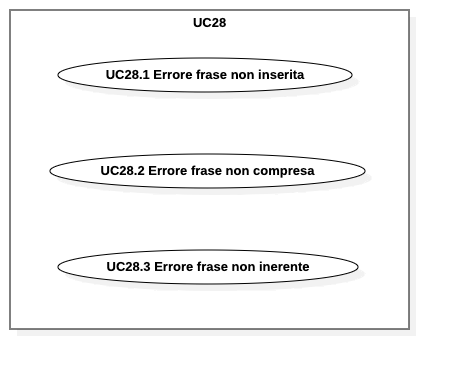
\includegraphics[scale=0.6]{UML_Use_Cases/UC28.1_28.2_28.3.png}
\begin{itemize}
	\item \textbf{Descrizione:} L’utente visualizza un errore relativo alla frase inserita;
	\item \textbf{Attori:} utente;
	\item \textbf{Precondizioni:} 
	\begin{itemize}
		\item L’utente ha selezionato un file di struttura \textit{Database} (\hyperref[sec:UC25]{\textbf{UC25}});
		\item L'utente ha inserito una frase in linguaggio naturale (\hyperref[sec:UC27]{\textbf{UC27}});
	\end{itemize}
	\item \textbf{Postcondizioni:} 
	\begin{itemize}
		\item Il programma mostra un messaggio di errore;
		\item Il \textit{prompt} non viene generato;
	\end{itemize}
	\item \textbf{Scenario principale:} 
	\begin{itemize}
		\item Il sistema non ha ricevuto una frase;
		\item Il sistema visualizza un messaggio di errore.
	\end{itemize}
\end{itemize}


\subsubsection{UC28.2 - Errore frase non compresa}
\label{sec:UC28.2}
\begin{itemize}
	\item \textbf{Descrizione:} L’utente inserisce una frase in linguaggio naturale non comprensibile dal sistema;
	\item \textbf{Attori:} utente;
	\item \textbf{Precondizioni:} 
	\begin{itemize}
		\item L’utente ha selezionato un file di struttura \textit{Database} (\hyperref[sec:UC25]{\textbf{UC25}});
		\item L'utente ha inserito una frase in linguaggio naturale (\hyperref[sec:UC27]{\textbf{UC27}});
	\end{itemize}
	\item \textbf{Postcondizioni:} 
	\begin{itemize}
		\item Il programma mostra un messaggio di errore;
		\item Il \textit{prompt} non viene generato;
	\end{itemize}
	\item \textbf{Scenario principale:} 
	\begin{itemize}
		\item Il sistema verifica la frase ricevuta;
		\item Il sistema non comprende la frase;
		\item Il sistema visualizza un messaggio di errore.
	\end{itemize}
\end{itemize}


\subsubsection{UC28.3 - Errore frase non inerente}
\label{sec:UC28.3}
%\includegraphics[]{diagramma_UML}
\begin{itemize}
	\item \textbf{Descrizione:} l’utente inserisce una frase in linguaggio naturale non interpretabile dal sistema come inerente al \textit{database};
	\item \textbf{Attori:} utente;
	\item \textbf{Precondizioni:} 
	\begin{itemize}
		\item L’utente ha selezionato un file di struttura \textit{Database} (\hyperref[sec:UC25]{\textbf{UC22}});
		\item L’utente ha scritto una frase in linguaggio naturale nella casella di testo apposita e ne ha confermato l’inserimento (\hyperref[sec:UC27]{\textbf{UC24}});
	\end{itemize}
	\item \textbf{Postcondizioni:} 
	\begin{itemize}
		\item Il programma mostra un messaggio di errore;
		\item Il \textit{prompt} non viene generato;
	\end{itemize}
	\item \textbf{Scenario principale:} 
	\begin{itemize}
		\item Il sistema verifica la frase ricevuta;
		\item Il sistema non trova componenti inerenti alla Struttura \textit{Database} nella frase;
		\item Il sistema visualizza un messaggio di errore.
	\end{itemize}
\end{itemize}

\subsection{UC29 - Visualizzazione \textit{prompt} generato}
\label{sec:UC29}
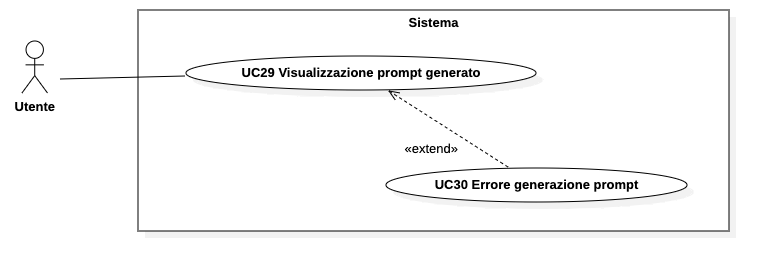
\includegraphics[scale=0.6]{UML_Use_Cases/UC29_30.png}
\begin{itemize}
	\item \textbf{Descrizione:} L’utente riceve il \textit{prompt} per la generazione della \textit{query};
	\item \textbf{Attori:} utente;
	\item \textbf{Precondizioni:} 
	\begin{itemize}
		\item L’utente ha selezionato un file di struttura \textit{Database} (\hyperref[sec:UC25]{\textbf{UC22}});
		\item L’utente ha scritto una frase in linguaggio naturale (\hyperref[sec:UC27]{\textbf{UC24}});
	\end{itemize}
	\item \textbf{Postcondizioni:} 
	\begin{itemize}
		\item Il programma visualizza il \textit{prompt} per la creazione della \textit{query} richiesta;
	\end{itemize}
	\item \textbf{Scenario principale:} 
	\begin{itemize}
		\item L’utente ha il programma aperto;
		\item L’utente ha selezionato la Struttura \textit{Database} (\hyperref[sec:UC25]{\textbf{UC25}})
		\item L'utente ha inserito la frase in linguaggio naturale (\hyperref[sec:UC27]{\textbf{UC27}});
		\item L’utente richiede il \textit{prompt};
		\item Il programma visualizza il \textit{prompt} elaborato.
	\end{itemize}
	\item \textbf{Estensioni:} nel caso in cui non sia possibile generare il \textit{prompt}:
	\begin{itemize}
		\item Viene visualizzato un errore - \hyperref[sec:UC30]{\textbf{UC30}}.
	\end{itemize}
\end{itemize}

\subsection{UC30 - Errore generazione \textit{prompt}}
\label{sec:UC30}
\begin{itemize}
	\item \textbf{Descrizione:} L’utente visualizza un errore inerente alla generazione del \textit{prompt};
	\item \textbf{Attori:} utente;
	\item \textbf{Precondizioni:} 
	\begin{itemize}
		\item L’utente ha selezionato un file di struttura \textit{Database} (\hyperref[sec:UC25]{\textbf{UC25}});
		\item L’utente ha scritto una frase in linguaggio naturale (\hyperref[sec:UC27]{\textbf{UC27}});
		\item L’utente richiede il \textit{prompt};
	\end{itemize}
	\item \textbf{Postcondizioni:} 
	\begin{itemize}
		\item L’utente visualizza un messaggio di errore;
	\end{itemize}
	\item \textbf{Scenario principale:} 
	\begin{itemize}
		\item Il sistema verifica il \textit{prompt} e ritorna l'errore adeguato;
	\end{itemize}
\end{itemize}

\subsubsection{UC30.1 - Errore comunicazione con \textit{LLM}}
\label{sec:UC30.1}
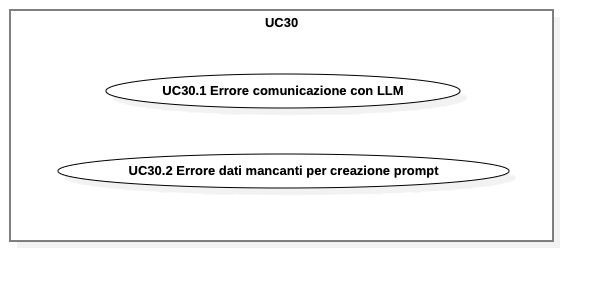
\includegraphics[scale=0.6]{UML_Use_Cases/UC30.1_30.2.png}
\begin{itemize}
	\item \textbf{Descrizione:} L’utente visualizza un errore inerente alla comunicazione con il modello \textit{LLM};
	\item \textbf{Attori:} utente;
	\item \textbf{Precondizioni:} 
	\begin{itemize}
		\item L’utente ha selezionato un file di struttura \textit{Database} (\hyperref[sec:UC25]{\textbf{UC25}});
		\item L’utente ha scritto una frase in linguaggio naturale (\hyperref[sec:UC27]{\textbf{UC27}});
		\item L’utente richiede il \textit{prompt};
	\end{itemize}
	\item \textbf{Postcondizioni:} 
	\begin{itemize}
		\item L’utente visualizza un messaggio di errore;
	\end{itemize}
	\item \textbf{Scenario principale:} 
	\begin{itemize}
		\item Il sistema riceve il \textit{prompt};
		\item Il sistema non riesce a comunicare con il modello \textit{LLM};
		\item Il sistema mostra un errore;
	\end{itemize}
\end{itemize}

\subsubsection{UC30.2 - Errore dati mancanti per creazione \textit{prompt}}
\label{sec:UC30.2}
\begin{itemize}
	\item \textbf{Descrizione:} L’utente visualizza un errore inerente alla frase in linguaggio naturale;
	\item \textbf{Attori:} utente;
	\item \textbf{Precondizioni:} 
	\begin{itemize}
		\item L’utente ha selezionato un file di struttura \textit{Database} (\hyperref[sec:UC25]{\textbf{UC25}});
		\item L’utente ha scritto una frase in linguaggio naturale (\hyperref[sec:UC27]{\textbf{UC27}});
		\item L’utente richiede il \textit{prompt};
	\end{itemize}
	\item \textbf{Postcondizioni:} 
	\begin{itemize}
		\item L’utente visualizza un messaggio di errore;
	\end{itemize}
	\item \textbf{Scenario principale:} 
	\begin{itemize}
		\item Il sistema riceve il \textit{prompt};
		\item Il sistema non trova tutti i dati necessari per la generazione del \textit{prompt} ;
		\item Il sistema mostra un errore;
	\end{itemize}
\end{itemize}

\subsection{UC31 - Richiesta generazione \textit{query SQL}}
\label{sec:UC31}
\includegraphics[scale=0.55]{UML_Use_Cases/UC31_32.png}
\begin{itemize}
    \item \textbf{Descrizione:} L'utente richiede la generazione della \textit{query SQL};
    \item \textbf{Attori:} utente;
    \item \textbf{Precondizioni:} 
    \begin{itemize}
    	\item L'utente ha visualizzato il \textit{prompt} (\hyperref[sec:UC29]{\textbf{UC29}});
    \end{itemize}
    \item \textbf{Postcondizioni:} 
    \begin{itemize}
    	\item L'utente visualizza la \textit{query SQL} richiesta (\hyperref[sec:UC33]{\textbf{UC33}});
    \end{itemize}
    \item \textbf{Scenario principale:}
    \begin{itemize}
    	\item L'utente richiede la generazione della \textit{query SQL} a partire dal \textit{prompt} ricevuto;
    	\item Il sistema verifica il \textit{prompt} ricevuto;
    	\item Il sistema invia il \textit{prompt} al servizio \textit{LLM} esterno;
    \end{itemize}
    \item \textbf{Estensioni:} In caso non sia possibile generare la \textit{query SQL}:
    \begin{itemize}
    	\item Errore generazione \textit{query SQL} (\hyperref[sec:UC32]{\textbf{UC32}});
    \end{itemize}
\end{itemize}

\subsection{UC32 - Errore generazione \textit{query SQL}}
\label{sec:UC32}
%   \includegraphics[]{diagramma_UML}
\begin{itemize}
	\item \textbf{Descrizione:} L'utente visualizza un messaggio di errore inerente alla generazione della \textit{query SQL};
	\item \textbf{Attori:} utente;
	\item \textbf{Precondizioni:} 
	\begin{itemize}
		\item L'utente ha visualizzato il \textit{prompt} (\hyperref[sec:UC29]{\textbf{UC29}});
		\item L'utente richiede la generazione della \textit{query SQL} (\hyperref[sec:UC31]{\textbf{UC31}});
	\end{itemize}
	\item \textbf{Postcondizioni:} 
	\begin{itemize}
		\item L'utente un messaggio di errore;
	\end{itemize}
	\item \textbf{Scenario principale:}
	\begin{itemize}
		\item L'utente richiede la generazione della \textit{query SQL} a partire dal \textit{prompt} ricevuto;
		\item Il sistema verifica il \textit{prompt} ricevuto;
		\item Il sistema invia il \textit{prompt} al servizio \textit{LLM} esterno;
		\item Il sistema mostra un messaggio di errore;
	\end{itemize}
\end{itemize}

\subsubsection{UC32.1 - Errore comunicazione con API}
\label{sec:UC32.1}
\includegraphics[scale=0.6]{UML_Use_Cases/UC32.1_32.2.png}
\begin{itemize}
	\item \textbf{Descrizione:} L'utente visualizza un messaggio di errore inerente alla comunicazione con il servizio di API esterno;
	\item \textbf{Attori:} utente;
	\item \textbf{Precondizioni:} 
	\begin{itemize}
		\item L'utente ha visualizzato il \textit{prompt} (\hyperref[sec:UC29]{\textbf{UC29}});
		\item L'utente richiede la generazione della \textit{query SQL} (\hyperref[sec:UC31]{\textbf{UC31}});
	\end{itemize}
	\item \textbf{Postcondizioni:} 
	\begin{itemize}
		\item L'utente un messaggio di errore;
	\end{itemize}
	\item \textbf{Scenario principale:}
	\begin{itemize}
		\item L'utente richiede la generazione della \textit{query SQL} a partire dal \textit{prompt} ricevuto;
		\item Il sistema verifica il \textit{prompt} ricevuto;
		\item Il sistema invia il \textit{prompt} al servizio \textit{LLM} esterno;
		\item Il sistema non riesce a comunicare con il servizio \textit{LLM} esterno;
		\item Il sistema mostra un messaggio di errore;
	\end{itemize}
\end{itemize}

\subsubsection{UC32.2 - Errore formattazione \textit{prompt}}
\label{sec:UC32.2}
\begin{itemize}
	\item \textbf{Descrizione:} L'utente visualizza un messaggio di errore inerente alla formattazione del \textit{prompt} creato;
	\item \textbf{Attori:} utente;
	\item \textbf{Precondizioni:} 
	\begin{itemize}
		\item L'utente ha visualizzato il \textit{prompt} (\hyperref[sec:UC29]{\textbf{UC29}});
		\item L'utente richiede la generazione della \textit{query SQL} (\hyperref[sec:UC31]{\textbf{UC31}});
	\end{itemize}
	\item \textbf{Postcondizioni:} 
	\begin{itemize}
		\item L'utente visualizza un messaggio di errore;
	\end{itemize}
	\item \textbf{Scenario principale:}
	\begin{itemize}
		\item L'utente richiede la generazione della \textit{query SQL} a partire dal \textit{prompt} ricevuto;
		\item Il sistema verifica il \textit{prompt} ricevuto;
		\item Il sistema invia il \textit{prompt} al servizio \textit{LLM} esterno;
		\item Il sistema riceve un errore dal servizio \textit{LLM} esterno;
		\item Il sistema mostra un messaggio di errore;
	\end{itemize}
\end{itemize}

\subsection{UC33 - Visualizzazione \textit{query SQL}}
\label{sec:UC33}
\begin{itemize}
	\item \textbf{Descrizione:} L’utente visualizza la \textit{query SQL} ricevuta dal servizio \textit{LLM} esterno;
	\item \textbf{Attori:} utente;
	\item \textbf{Precondizioni:} 
	\begin{itemize}
		\item L’utente ha selezionato un file di struttura \textit{Database} (\hyperref[sec:UC25]{\textbf{UC25}});
		\item L’utente ha inserito una frase in linguaggio naturale (\hyperref[sec:UC27]{\textbf{UC27}});
		\item Il programma visualizza il \textit{prompt} elaborato (\hyperref[sec:UC29]{\textbf{UC29}});
		\item L’utente richiesto la generazione della \textit{query SQL} (\hyperref[sec:UC31]{\textbf{UC31}});
	\end{itemize}
	\item \textbf{Postcondizioni:} 
	\begin{itemize}
		\item Il programma visualizza la \textit{query SQL} richiesta;
	\end{itemize}
	\item \textbf{Scenario principale:} 
	\begin{itemize}
		\item L'utente richiede la generazione della \textit{query SQL} (\hyperref[sec:UC31]{\textbf{UC31}});
		\item L'utente visualizza la \textit{query SQL} richiesta;
	\end{itemize}
\end{itemize}


\section{Requisiti}
\subsection{Requisiti funzionali}
\subsection{Requisiti di qualità}
\subsection{Requisiti di vincolo}
\subsection{Tracciamento}


\end{document}